\documentclass[a4paper]{scrartcl}
\usepackage[utf8]{inputenc}
\usepackage[english]{babel}
\usepackage{graphicx}
\usepackage{lastpage}
\usepackage{pgf}
\usepackage{wrapfig}
\usepackage{fancyvrb}
\usepackage{fancyhdr}
\pagestyle{fancy}

% Create header and footer
\usepackage[backend=bibtex, citestyle=numeric-comp, bibstyle=ieee]{biblatex}
\addbibresource{ref.bib} % The file containing our references, in BibTeX format
\usepackage{hyperref}
\usepackage{listings}
\usepackage{subcaption}
\usepackage{enumitem}
\usepackage[section]{placeins}

% Create header and footer
\headheight 27pt
\pagestyle{fancyplain}
\lhead{\footnotesize{Internet Applications, ID1354}}
\chead{\footnotesize{Tasty Recipes with JavaScript}}
\rhead{}
\lfoot{}
\cfoot{\thepage\ (\pageref{LastPage})}
\rfoot{}

% Create title page
\title{Tasty Recipes with JavaScript}
\subtitle{Internet Applications, ID1354}
\author{Julius Recep Colliander Celik - jcelik@kth.se}
\date{\today}

\begin{document}

\maketitle

\section*{Tips for Report Writing}
\textbf{REMOVE THIS SECTION BEFORE SUBMITTING THE REPORT.}\\

\noindent \textit{The target audience has exactly the same skills as the author, except they do not know anything at all about the specific program described in the report.} \\

Consider the following:

\begin{itemize}
  \item \textbf{The report must be \textit{centered around the requirements}. Which are they (Introduction), how did you work to meet them (Method), what is the solution that meets them (Result), and how can you be sure they are met (Discussion). This is the IMRaD method.}

  \item \textbf{The report must show that you have done the work yourself and that you have understood what you have done. Both of these goals are met by carefully explaining the source code.}

  \item Is spelling and grammar correct? Is spoken language avoided?

  \item Does the report have a good structure with sections, subsections and paragraphs?

  \item Is the solution clearly explained? Will the reader understand the program? What would you yourself want to know if you read about the program, is that included in the report?

  \item Is the solution analyzed and evaluated? Are important properties of the program explained? Should there have been more extensive evaluation?

  \item Is the text clarified with images and/or other figures, and with links to the code in your Git repository? Remember that all figures (images, tables, graphs, code listings, etc) shall be numbered and have a short explaining text.
\end{itemize}

\section{Introduction}

This assignment was a continuation of the last one, where front-end interactivity was added to create a more fluent experience. Specifically JavaScript was used to introduce asynchronous interactions, where the window did not have to refresh for actions to be visible. The JavaScript framework React was used. To view the website it is publicly available on the link \href{https://github.com/juliuscc/kth-id1354/tree/master/homework-4}{https://github.com/juliuscc/kth-id1354/tree/master/homework-4}.

\section{Literature Study}

The React documentation was used for reference \href{https://reactjs.org/docs/}{https://reactjs.org/docs/}.

\section{Method}

I reused the code from the first assignment and modified it to achieve the tasks in this lab. I used VS Code as my text editor and used MAMP as a PHP web server and Database. I also introduced a Create React App project for development which later was extracted into another project that could enable the code to be used separately as a module on the page. Insomnia was used when developing the back-end API.

\section{Result}

I used the front-end framework React to implement a viewmodel sub-application, as I am familiar with React. To easily use one React app, instead of multiple apps that communicated with each other, I moved the login and register functionality to the comment section. Figure \ref{fig:comment-section} shows how the React app looks in different states.

\begin{figure}
	\centering
	\begin{subfigure}[b]{0.3\linewidth}
			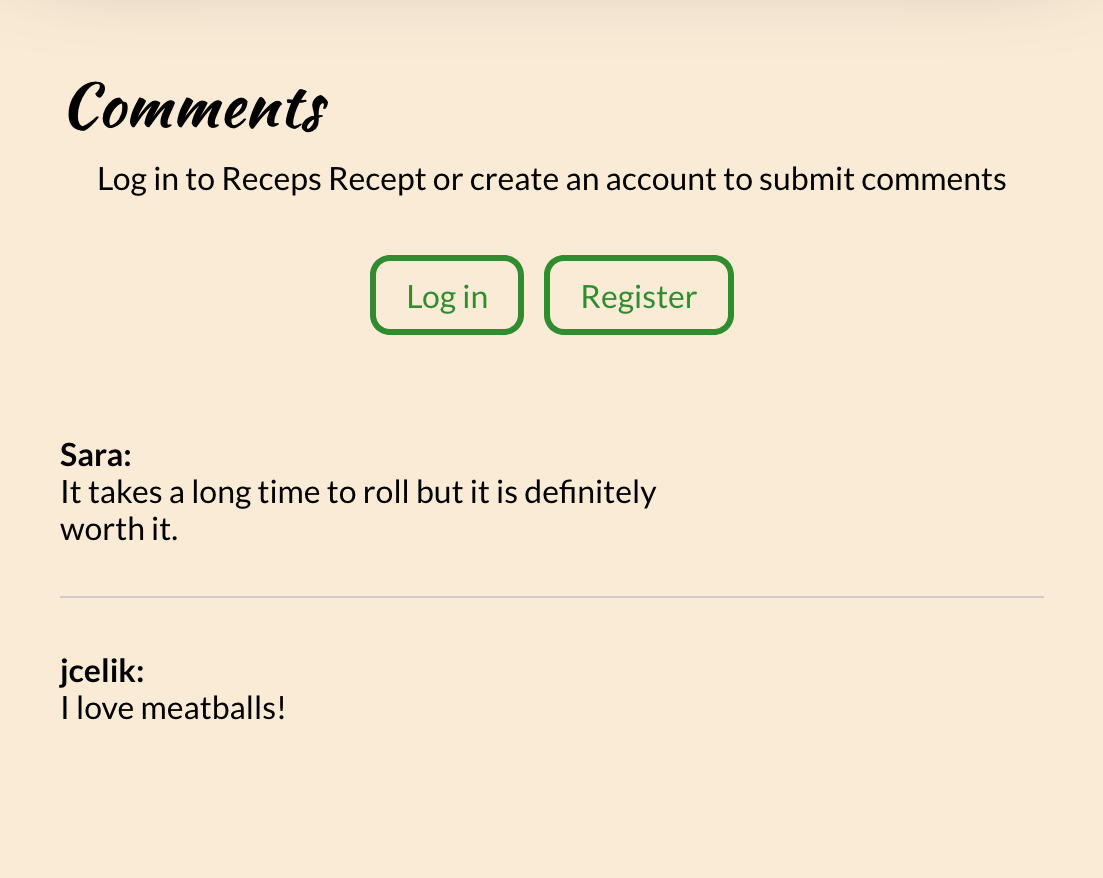
\includegraphics[width=\linewidth]{images/screenshot-comments-logged_out.png}
			\caption{Comment section with no user logged in.}
	\end{subfigure}
	\begin{subfigure}[b]{0.3\linewidth}
		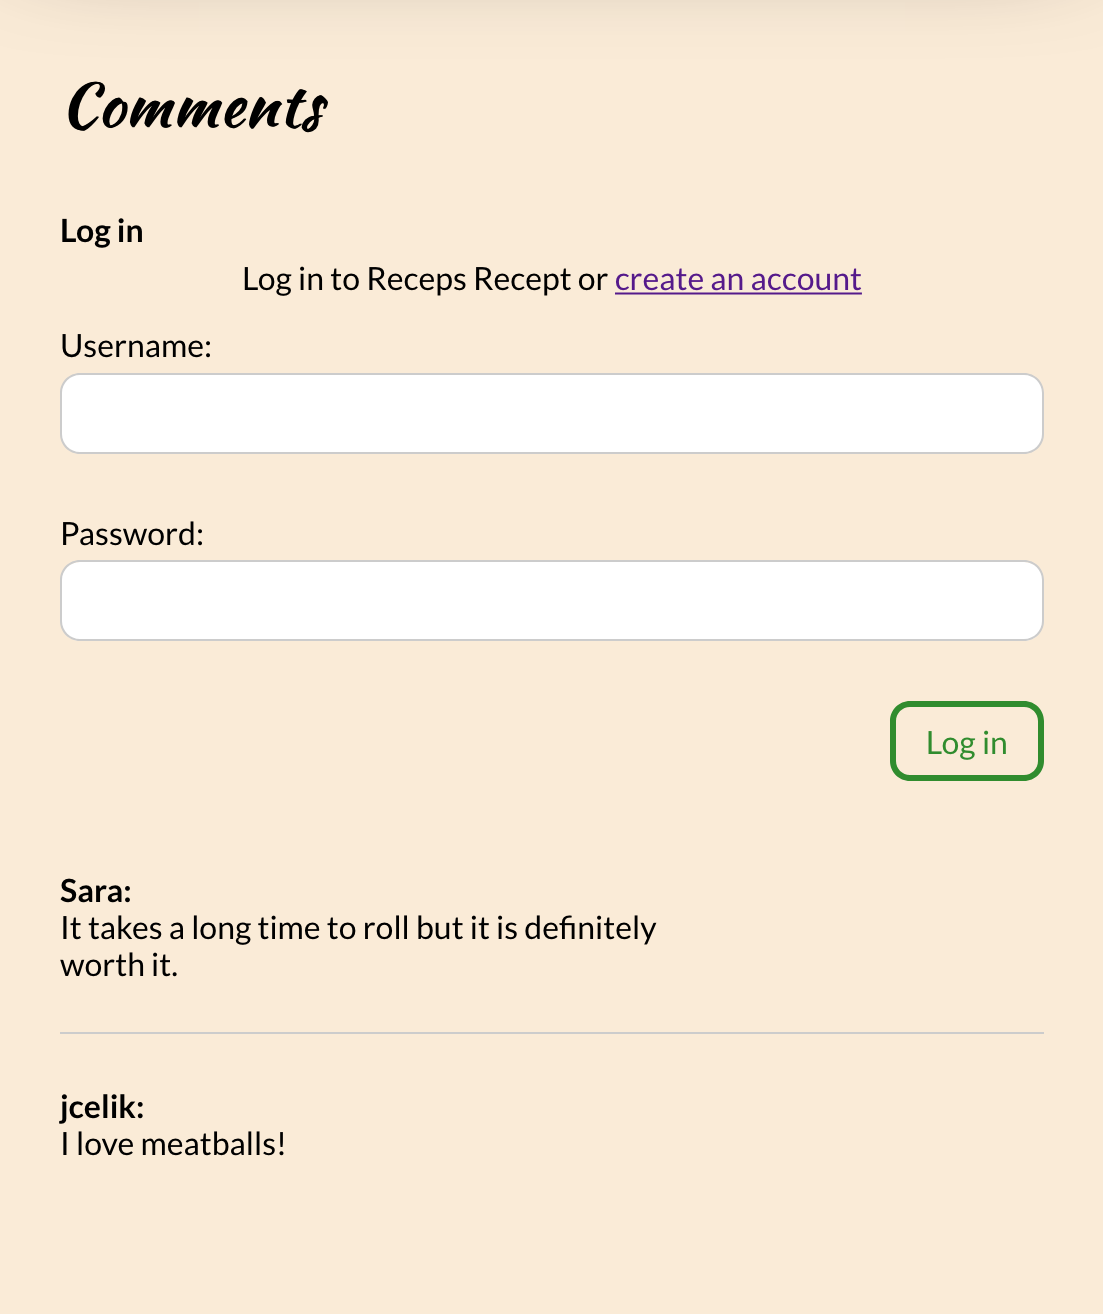
\includegraphics[width=\linewidth]{images/screenshot-comments-login.png}
		\caption{Comment section when logging in.}
	\end{subfigure}
	\begin{subfigure}[b]{0.3\linewidth}
		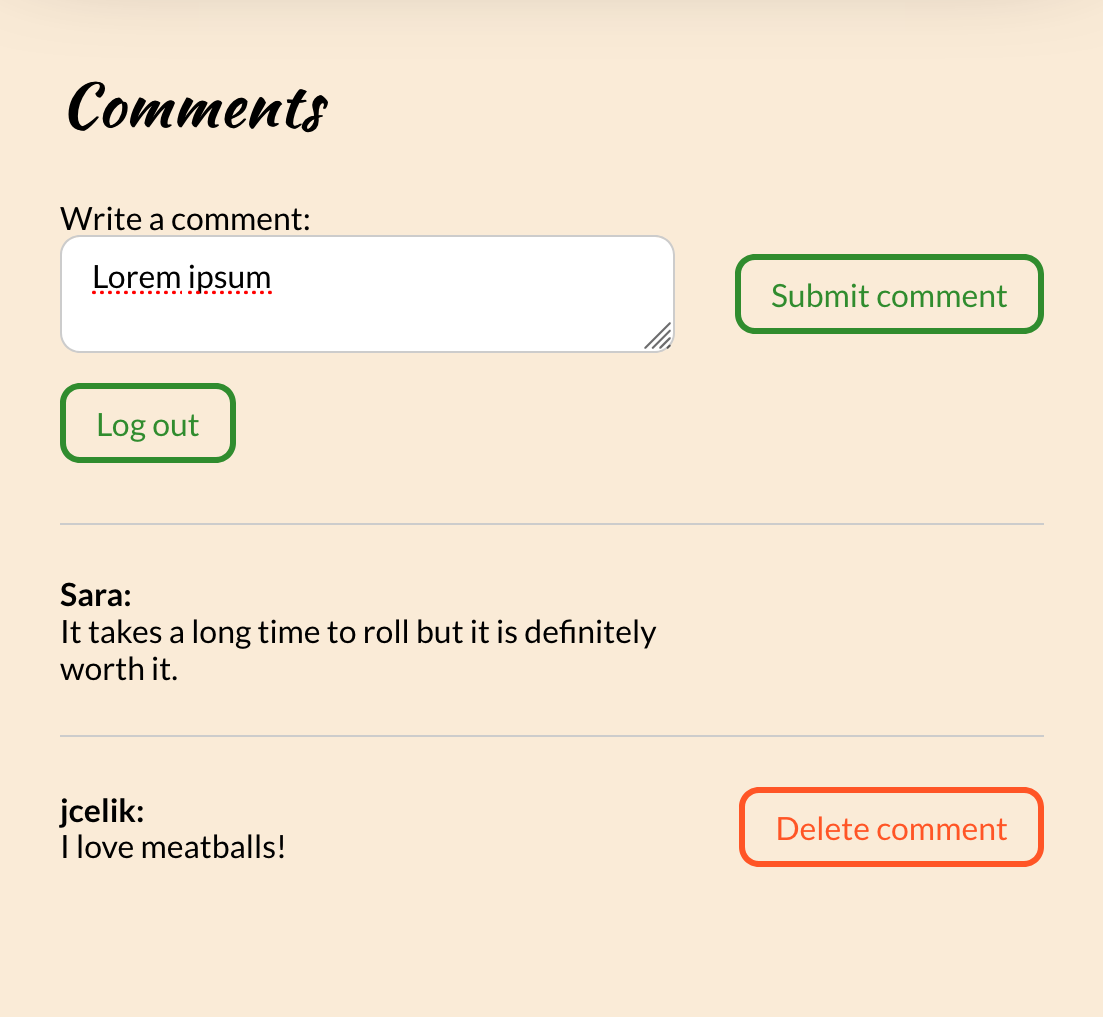
\includegraphics[width=\linewidth]{images/screenshot-comments-logged_in.png}
		\caption{Comment section when user is logged in.}
	\end{subfigure}
	\caption{Comment section with authentication implemented with React.}
	\label{fig:comment-section}
\end{figure}

\section{Fetch instead of AJAX}

\section{Fetch for authentication}

\section{Storing authentication tokens}

\section{Data sent from server}

\section{The viewmodel}

%\begin{itemize}
%\item The report must show that AJAX is used for login and logout; and reading, writing and deleting recipe comments.
%\item The report must show that there is a viewmodel, and that it is managed by Knockout (or another JavaScript framework).
%\item The report must show that no HTML code, but only data, is sent in response to an AJAX request.
%
%\end{itemize}

\section{Discussion}

\textbf{This section \textit{analysis} the result presented in the previous section.} \\

\noindent Summarize the requirements and \textit{clearly state which of them you have met}. What lessons have you learned and what problems did you face? How were the problems solved? Should you have done something differently?

\section{Comments About the Course}

Any comment(s) related to this course offering or to coming offerings is much appreciated. \textit{Please also tell approximately how much time you spent on the assignment}, including lectures and exercises. This is of great help for course evaluation.

\end{document}
